\documentclass{beamer}
\usepackage[spanish]{babel}
\usepackage[utf8]{inputenc}
\usepackage{graphicx}
\graphicspath{ {./images/}}

\usetheme{Madrid}
\usecolortheme{default}

%------------------------------------------------------------
%This block of code defines the information to appear in the
%Title page
\title[PC1 Estadistica Aplicada] %optional
{Aplicacion de tecnicas de estimacion y prueba de hipotesis}

\subtitle{
  Caso: tendencias socio-economicas de algunas
  lineas de carrea de Ingenieria de sistemas
}

\author % (optional)
{
  Alvarez \and Bautista \and Burga \and
  Casanova \and  Cuyate
}

\institute
{
  Facultad de Ingenieria Industrial y de Sistemas\\
  \textbf{Universidad Nacional de Ingenieria}
}

\date
{Octubre 2022}

% \logo{\includegraphics[height=1cm]{overleaf-logo}}

%End of title page configuration block
%------------------------------------------------------------

%------------------------------------------------------------
%The next block of commands puts the table of contents at the
%beginning of each section and highlights the current section:

\AtBeginSection[]
{
  \begin{frame}
    \frametitle{Tabla de Contenido}
    \tableofcontents[currentsection]
  \end{frame}
}
%------------------------------------------------------------


\begin{document}

%The next statement creates the title page.
\frame{\titlepage}


%---------------------------------------------------------
%This block of code is for the table of contents after
%the title page
\begin{frame}
\frametitle{Tabla de Contenido}
\tableofcontents
\end{frame}
%---------------------------------------------------------

\section{Problema}

\begin{frame}
\frametitle{Problematica}

\begin{itemize}
    \item Empiricamente se observa que en el mundo la precarizacion del trabajo
se acrecenta cada vez mas, de igual modo con la evolucion
    de personas casadas y los salarios promedio de los jovenes
    \item Con motivo de generar informacion util para la prediccion de estas tendencias
socio-economicas se ha procedio a realizar un analisis estadistico sobre
9 hipotesis planteadas

\end{itemize}
\end{frame}



%---------------------------------------------------------
\section{Objetivos}

%---------------------------------------------------------
\begin{frame}

\frametitle{Objetivos del trabajo}

\begin{alertblock}{General}
  Generar informacion relevante para la prediccion de tendencias
  socio-economicas en el mundo tomando como referencia datos
  provenientes de distintos paises.
\end{alertblock}
\end{frame}

\begin{frame}
\frametitle{Hipotesis especificas}

\begin{columns}
\column{0.5\textwidth}

  \begin{itemize}
      \item La distribucion de ingresos de  sigue
        la ley normal
      \item La eleccion de especialidad es causa de la formacion de 2 grupos
        en la poblacion.
      \item Las personas que trabajan una cantidad de horas superior a
        la media tienen una mejor destribucion de ingresos que aquellas
        que no lo hacen
  \end{itemize}

\column{0.5\textwidth}

  \begin{itemize}
      \item En paises desarrollados existe una mayor cantidad
        de mujeres con puestos de trabajos relacionados a ingenieria que en paises en via
        de desarrollo
      \item Los cientificos de datos poseen un mejor distribucion de ingresos
        que los ingenieros de datos
      \item El sector \textit{(publico / privado)} al que pertenece un trabajador
        es causa de la diferencia de salarios
  \end{itemize}
\end{columns}
\end{frame}

%---------------------------------------------------------

\begin{frame}
\frametitle{Hipotesis especificas}
  \begin{itemize}
      \item El \alert{promedio de ingresos} de las personas que trabajan
        una cantidad de horas superior a la mediana es mayor al promedio
        de ingreso de personas que laburan una cantidad menor de horas
        que la mediana
      \item Las personas de mediana edad poseen una mejor distribucion
        de ingreso que las personas jovenes
      \item El promedio de ingresos de la poblacion mexicana es mayor
        que la peruana
  \end{itemize}

  \textbf{Cada hipotesis tiene asociado el objetivo de comprobar
  o rechazar la suposicion}

\end{frame}

%---------------------------------------------------------


%---------------------------------------------------------
\section{Importancia de los objetivos}

\begin{frame}
  \textbf{\textit{
    Acerca de la normalidad de la distribucion de ingesos
  }}
  \\
  \alert{Ever no te olvides del texto}
  \newline

  \textit{\textbf{
    Sobre la eleccion de especialidad
  }}

  % \newline

  Se desea analizar principalmente:

  \begin{enumerate}
      \item Si la eleccion de la especializacion es causa de la
        formacion de 2 clusters en la poblacion

      \item Que tan confiable resulta usar \textbf{ANOVA} \footnotemark
  \end{enumerate}
  \footnotetext[1]{\textit{Analysis of Variance}}


\end{frame}

\begin{frame}
  \textit{\textbf{
    Sobre los demas objetivos
  }}
  \newline

  Se consideraron las hipotesis de tal forma que brinde
  información relevante para el análisis del mercado laboral
  para los egresados de la carrera de \textit{Ingenieria de
  sistemas}

\end{frame}

%---------------------------------------------------------


\section{Resultados y Conclusiones}

\begin{frame}
  \frametitle{Hipotesis 1}
  \begin{figure}[t]
    \caption{Data sin estandarizar}
    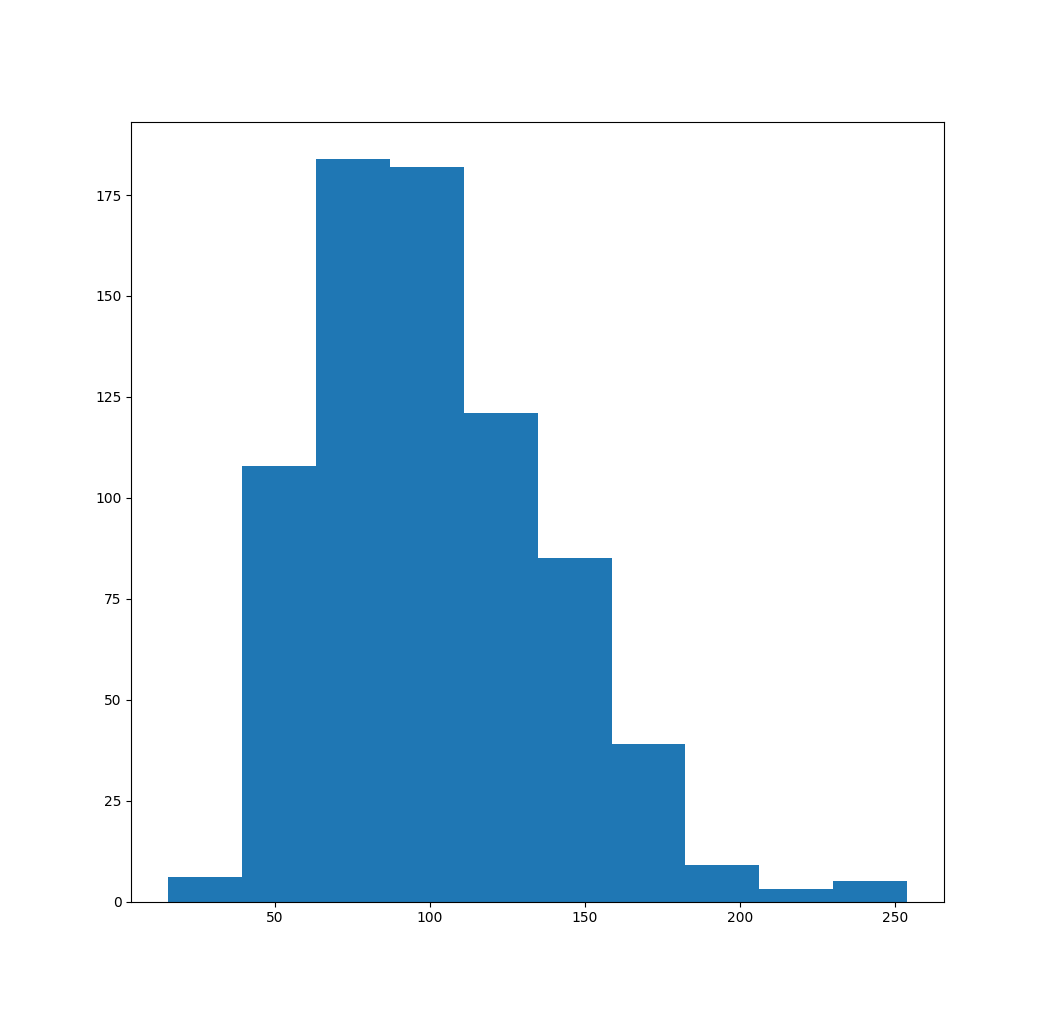
\includegraphics[width=5cm]{Figure_1.png}
  \end{figure}

\end{frame}

\begin{frame}
\frametitle{Hipotesis 1}
\begin{figure}[t]
  \caption{Data estandarizada y sin outliers}
  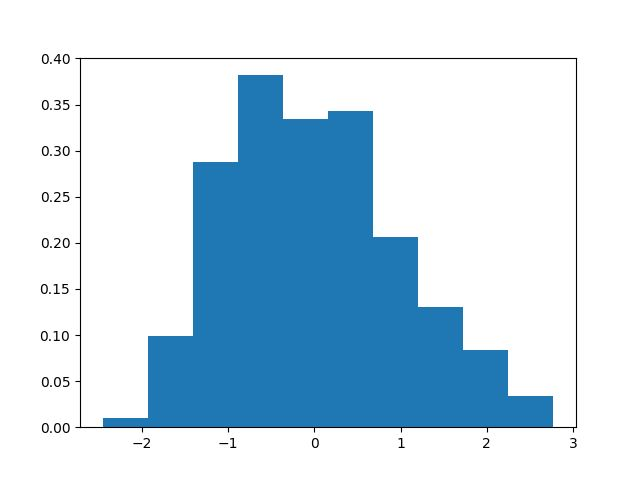
\includegraphics[width=6cm]{data_sin_outliers.jpeg}
\end{figure}
  \textbf{Puede parecer una distribucion Normal}

\end{frame}

\begin{frame}
\frametitle{Hipotesis 1}
\begin{figure}[t]
  \caption{Grafica Q-Q}
  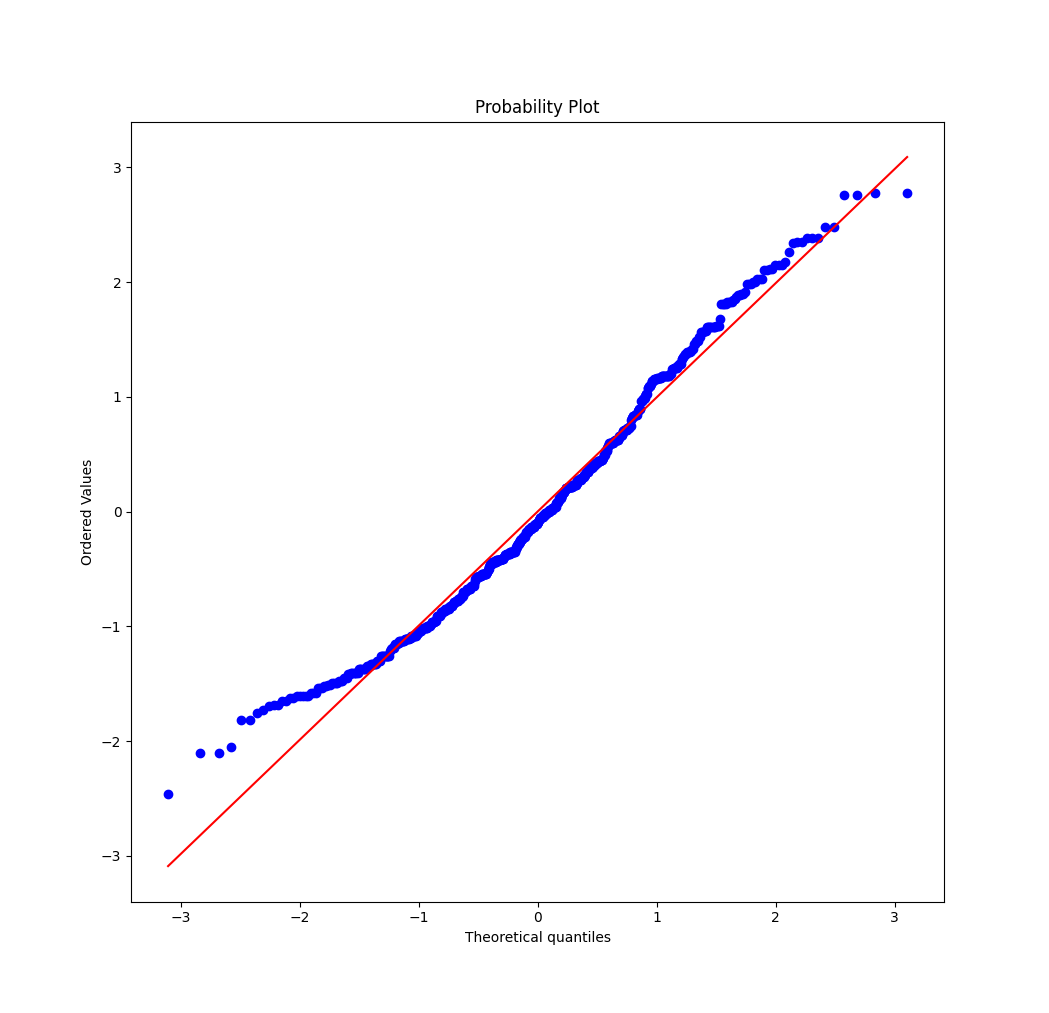
\includegraphics[width=6cm]{grafiaq-q.png}
\end{figure}

  \textbf{Se aleja de la distribucion normal}
\end{frame}

\begin{frame}

  Se aplicó el test de \textit{Jarque-Bera}, para comprobar si la muestra
  presenta una \textbf{curtosis} y \textbf{asimetria} correspondientes
  a una ley normal.

  El estadistico de \textit{Jarque Bera} es asintoticamente un estimador de
  una \textit{Chi-Cuadrado} (${\chi_n ^ 2}$) y toma como hipotesis nula que los datos de la
  muestra siguen la ley normal

  \begin{alertblock}{Test de Jarque-Bera}
    \[\textbf{JB} = \frac{n}{6}(S^2 +\frac{1}{4}(K - 3)^3)\] Siendo \textit{n} los grados de libertad
  \end{alertblock}

  \begin{block}{Estimadores de momentos centrales}
    \begin{itemize}
        \item Tercer Momento Central
          \[S = \frac{\hat{\mu}_3}{\hat{\sigma}^3}\]

        \item  Cuarto Momento Central
         \[K = \frac{\hat{\mu}_4}{\hat{\sigma}^4}\]
    \end{itemize}
  \end{block}
\end{frame}

\begin{frame}
  Adicionalmente, se usara el test de \textit{Kolmogorov-Smirnov}, donde se plantea
  que la distribucion de ingresos en la poblacion de ciencia de datos
  no sigue la ley normal y se comparará con la funcion acumulada teoria
  de esta

\end{frame}

\begin{frame}
\frametitle{Conclusiones hipotesis 1}
  El test K-S y el de Jarque-Bera muestran los siguientes p-values. 
\end{frame}


\begin{frame}
\frametitle{Hipotesis 2}
  Antes de realizar cualquier tecnica de inferencia es necesario conocer
  la forma de las distribuciones, incluso antes de analizar la varianza

\begin{figure}[h]
  \caption{Distribución de ingresos de ingenieros de
  software en la India}
  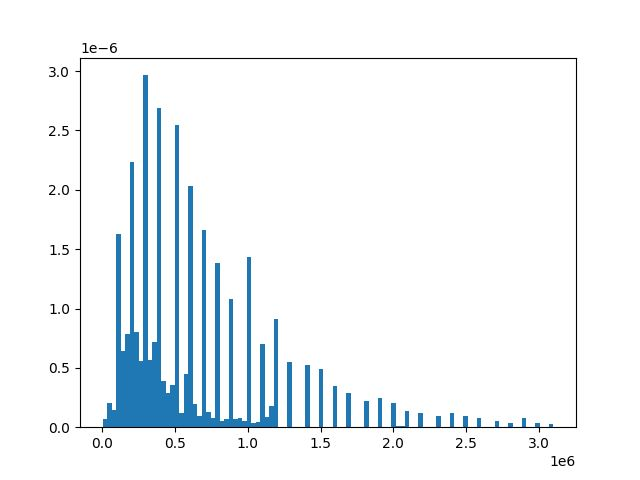
\includegraphics[width=6cm]{distribucion_ingresos_sw.jpeg}
\end{figure}

  se puede notar como existen \textit{2 grupos en la poblacion}
\end{frame}

\begin{frame}
  \frametitle{Distribución de los trabajadores en software}
  \alert{Aplicacion del test \textbf{Kolmogórov-Smirnov}}

  En este caso se va a comprar la funcion de distribucion acumulada observada
  con la de la distribucion teoria de una exponencial

\end{frame}

\begin{frame}
  \frametitle{Separando grupos aparentes}
  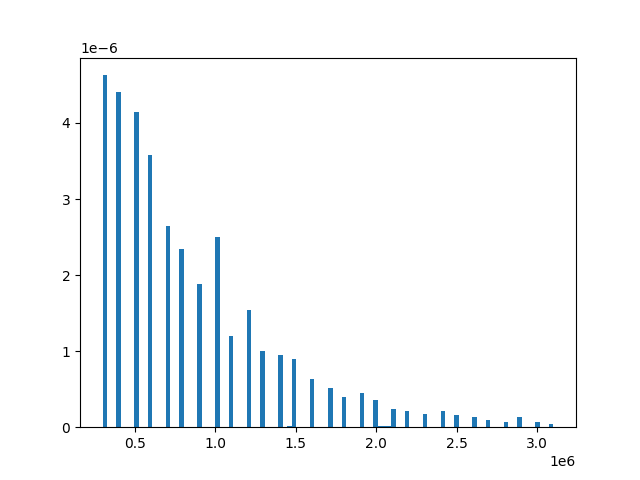
\includegraphics[width=8cm]{procesado.png}
  
\end{frame}

\begin{frame}
  \frametitle{Ajustando Curva}
  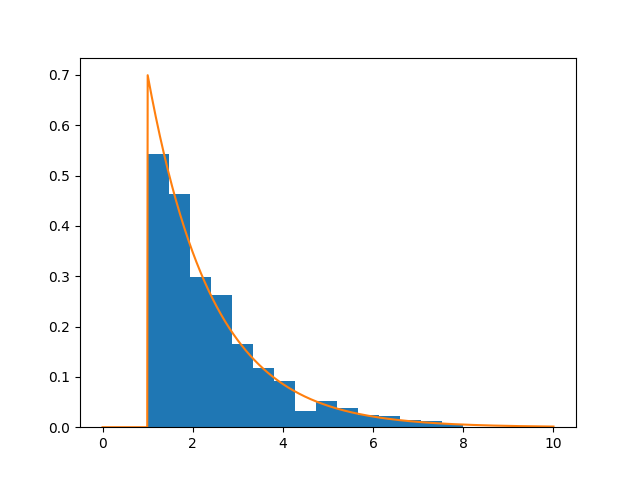
\includegraphics[width=8cm]{hip2/ajustando_curva.png}
  
\end{frame}

\begin{frame}
  \frametitle{Funciones acumuladas}
  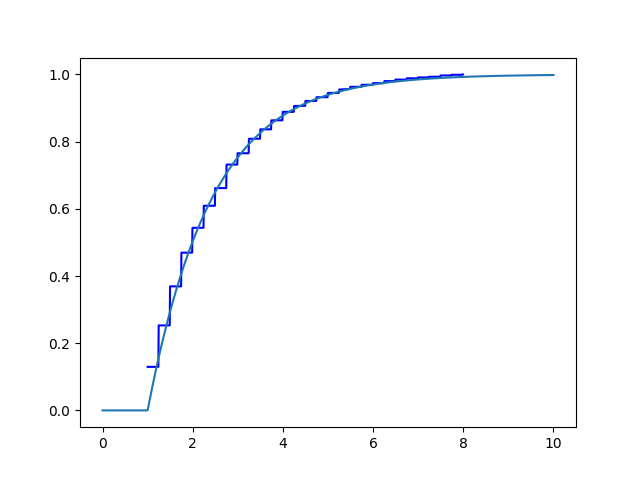
\includegraphics[width=8cm]{hip2/acumuladas.png}
  
\end{frame}

\begin{frame}
  \frametitle{Grafico P-P}
  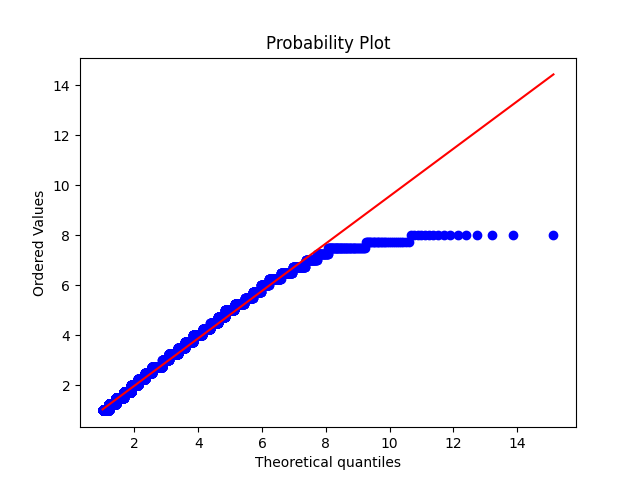
\includegraphics[width=8cm]{hip2/grafico_pp.png}
  
\end{frame}

\begin{frame}
  \frametitle{Conclusiones}
  De acuerdo al p-value obtenido no se puede rechazar la hipótesis nula
  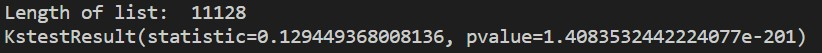
\includegraphics[width=9cm]{hip2/p-val.jpg}
\end{frame}
%\section{Conclusiones}

%%---------------------------------------------------------
%\begin{frame}
%\frametitle{Conclusiones}

%\begin{block}{Remark}
%Sample text
%\end{block}

%\begin{alertblock}{Important theorem}
%Sample text in red box
%\end{alertblock}

%\begin{examples}
%Sample text in green box. The title of the block is ``Examples".
%\end{examples}
%\end{frame}
%%---------------------------------------------------------


%%---------------------------------------------------------
%%Two columns
%\begin{frame}
%\frametitle{Two-column slide}

%\begin{columns}

%\column{0.5\textwidth}
%This is a text in first column.
%$$E=mc^2$$
%\begin{itemize}
%\item First item
%\item Second item
%\end{itemize}

%\column{0.5\textwidth}
%This text will be in the second column
%and on a second tought this is a nice looking
%layout in some cases.
%\end{columns}
%\end{frame}
%%---------------------------------------------------------

\end{document}
